%=============================================================
% Chapitre 6 — Résultats et interprétation
%=============================================================
\chapter{Résultats électoraux prédits et interprétation}
\label{ch:resultats}

\section{De la classe économique à l'orientation électorale}

Le passage des prédictions ML (classes économiques) aux scores électoraux s'effectue
via une table de correspondance \texttt{ECO\_TO\_ORIENTATION} et des poids intra-bloc
basés sur les résultats réels 2022 :

\begin{table}[H]
\centering
\caption{Mapping orientation électorale — 12 candidats du 1\textsuperscript{er} tour}
\label{tab:mapping}
\begin{tabular}{llp{7cm}}
\toprule
\textbf{Classe éco.} & \textbf{Bloc} & \textbf{Candidats (poids relatifs)} \\
\midrule
Boom       & Extrême-Gauche & Mélenchon 60\%, Roussel 20\%, Poutou 12\%, Arthaud 8\% \\
Croissance & Gauche         & Jadot 45\%, Hidalgo 35\%, Lassalle 20\% \\
Stable     & Centre         & Macron 80\%, Dupont-Aignan 12\%, Pécresse 8\% \\
Déclin     & Droite         & Pécresse 55\%, Zemmour 30\%, Dupont-Aignan 15\% \\
Crise      & Extrême-Droite & Le Pen 65\%, Zemmour 30\%, Asselineau 5\% \\
\bottomrule
\end{tabular}
\end{table}

\noindent Pour chaque département, la distribution des cantons prédits dans chaque classe
est pondérée par ce mapping pour produire un score par candidat.
Ces scores sont ensuite persistés dans la collection \texttt{predictions} de MongoDB,
qui constitue la source de vérité pour l'affichage dans le dashboard React.

\section{Prédictions départementales (HistGradientBoosting)}

\begin{table}[H]
\centering
\caption{Prédictions départementales — HistGradientBoosting vs réalité 2022}
\label{tab:dept_preds}
\begin{tabular}{llllr}
\toprule
\textbf{Département} & \textbf{Classe éco.} & \textbf{Vainqueur préd.} & \textbf{Score préd.} & \textbf{Correct} \\
\midrule
Charente           & Croissance & Macron & 41,5\% & \textcolor{green!60!black}{\checkmark} \\
Charente-Maritime  & Stable     & Macron & 64,6\% & \textcolor{green!60!black}{\checkmark} \\
Corrèze            & Stable     & Macron & 59,2\% & \textcolor{green!60!black}{\checkmark} \\
Creuse             & Stable     & Macron & 71,8\% & \textcolor{green!60!black}{\checkmark} \\
Deux-Sèvres        & Stable     & Macron & 75,2\% & \textcolor{green!60!black}{\checkmark} \\
Dordogne           & Stable     & Macron & 72,5\% & \textcolor{green!60!black}{\checkmark} \\
Gironde            & Stable     & Macron & 67,4\% & \textcolor{green!60!black}{\checkmark} \\
Haute-Vienne       & Stable     & Macron & 52,9\% & \textcolor{green!60!black}{\checkmark} \\
Landes             & Stable     & Macron & 73,2\% & \textcolor{green!60!black}{\checkmark} \\
\textbf{Lot-et-Garonne} & Stable & Macron & 67,7\% & \textcolor{red}{\textbf{$\times$}} \\
Pyrénées-Atlantiques & Stable   & Macron & 53,0\% & \textcolor{green!60!black}{\checkmark} \\
Vienne             & Stable     & Macron & 67,0\% & \textcolor{green!60!black}{\checkmark} \\
\midrule
\multicolumn{4}{l}{\textbf{Précision départementale}} & \textbf{91,7\% (11/12)} \\
\bottomrule
\end{tabular}
\end{table}

\begin{resultbox}[Précision départementale : 91,7\%]
Le modèle HistGradientBoosting prédit correctement le vainqueur dans
\textbf{11 des 12 départements}, soit une précision de \textbf{91,7\%}.
L'unique erreur concerne le Lot-et-Garonne, où la victoire de Marine Le Pen
(RN) n'est pas anticipée par le modèle.
\end{resultbox}

\section{Analyse de l'erreur — Lot-et-Garonne}

\begin{warnbox}[Erreur de prédiction — Lot-et-Garonne]
Le modèle prédit \textbf{Macron à 67,7\%} alors que c'est \textbf{Marine Le Pen} qui
arrive en tête dans ce département lors du 1\textsuperscript{er} tour 2022.

\textbf{Explication :} La classe économique prédite est \textit{Stable}, ce qui oriente
mécaniquement vers le Centre (Macron). Pourtant, les données 2022 révèlent :
\begin{itemize}
  \item Un chômage agricole structurel non capté par les $\Delta$-features (variation inter-
    recensements insuffisante pour refléter un malaise diffus de longue date)
  \item Une trajectoire de Le Pen déjà forte en 2017 (vote d'enracinement)
  \item Un biais du modèle synthétique : la classe \textit{Stable} est sur-représentée
    (40\% du dataset), ce qui écrase les nuances intra-classe
\end{itemize}

\textbf{Piste d'amélioration :} Intégrer des variables de vote historique (2017, 2019)
comme features supplémentaires pour capturer la composante identitaire du vote.
\end{warnbox}

\section{Prédiction régionale (agrégée)}

\begin{table}[H]
\centering
\caption{Scores régionaux agrégés (Nouvelle-Aquitaine) — comparaison des 5 modèles}
\label{tab:regional}
\begin{tabular}{llr}
\toprule
\textbf{Modèle} & \textbf{Vainqueur prédit} & \textbf{Score Macron} \\
\midrule
LogisticRegression          & Macron & 97,1\% \\
\rowcolor{green!15}
\textbf{HistGradientBoosting} & Macron & \textbf{68,7\%} \\
LinearSVM                   & Macron & 61,3\% \\
XGBoost                     & Macron & 59,3\% \\
RandomForest                & Macron & 56,1\% \\
\midrule
\textit{Résultat réel 2022} & Macron & \textit{$\sim$30\%} \\
\bottomrule
\end{tabular}
\end{table}

\noindent Le score HistGradientBoosting (68,7\%) surévalue Macron par rapport
au résultat réel ($\sim$30\% au 1\textsuperscript{er} tour), mais place correctement
Macron en 1\textsuperscript{er}, suivi de Pécresse (10,0\%) et Mélenchon (9,7\%).
La surestimation est inhérente au biais de la classe \textit{Stable} dans la variable
cible synthétique.

\begin{resultbox}[Podium régional prédit (HistGradientBoosting)]
\begin{center}
\large
1\textsuperscript{er} : \textbf{Macron} — 68,7\% \quad
2\textsuperscript{e} : Pécresse — 10,0\% \quad
3\textsuperscript{e} : Mélenchon — 9,7\%
\end{center}
\end{resultbox}

\section{Distribution des orientations par département}

\begin{figure}[H]
  \centering
  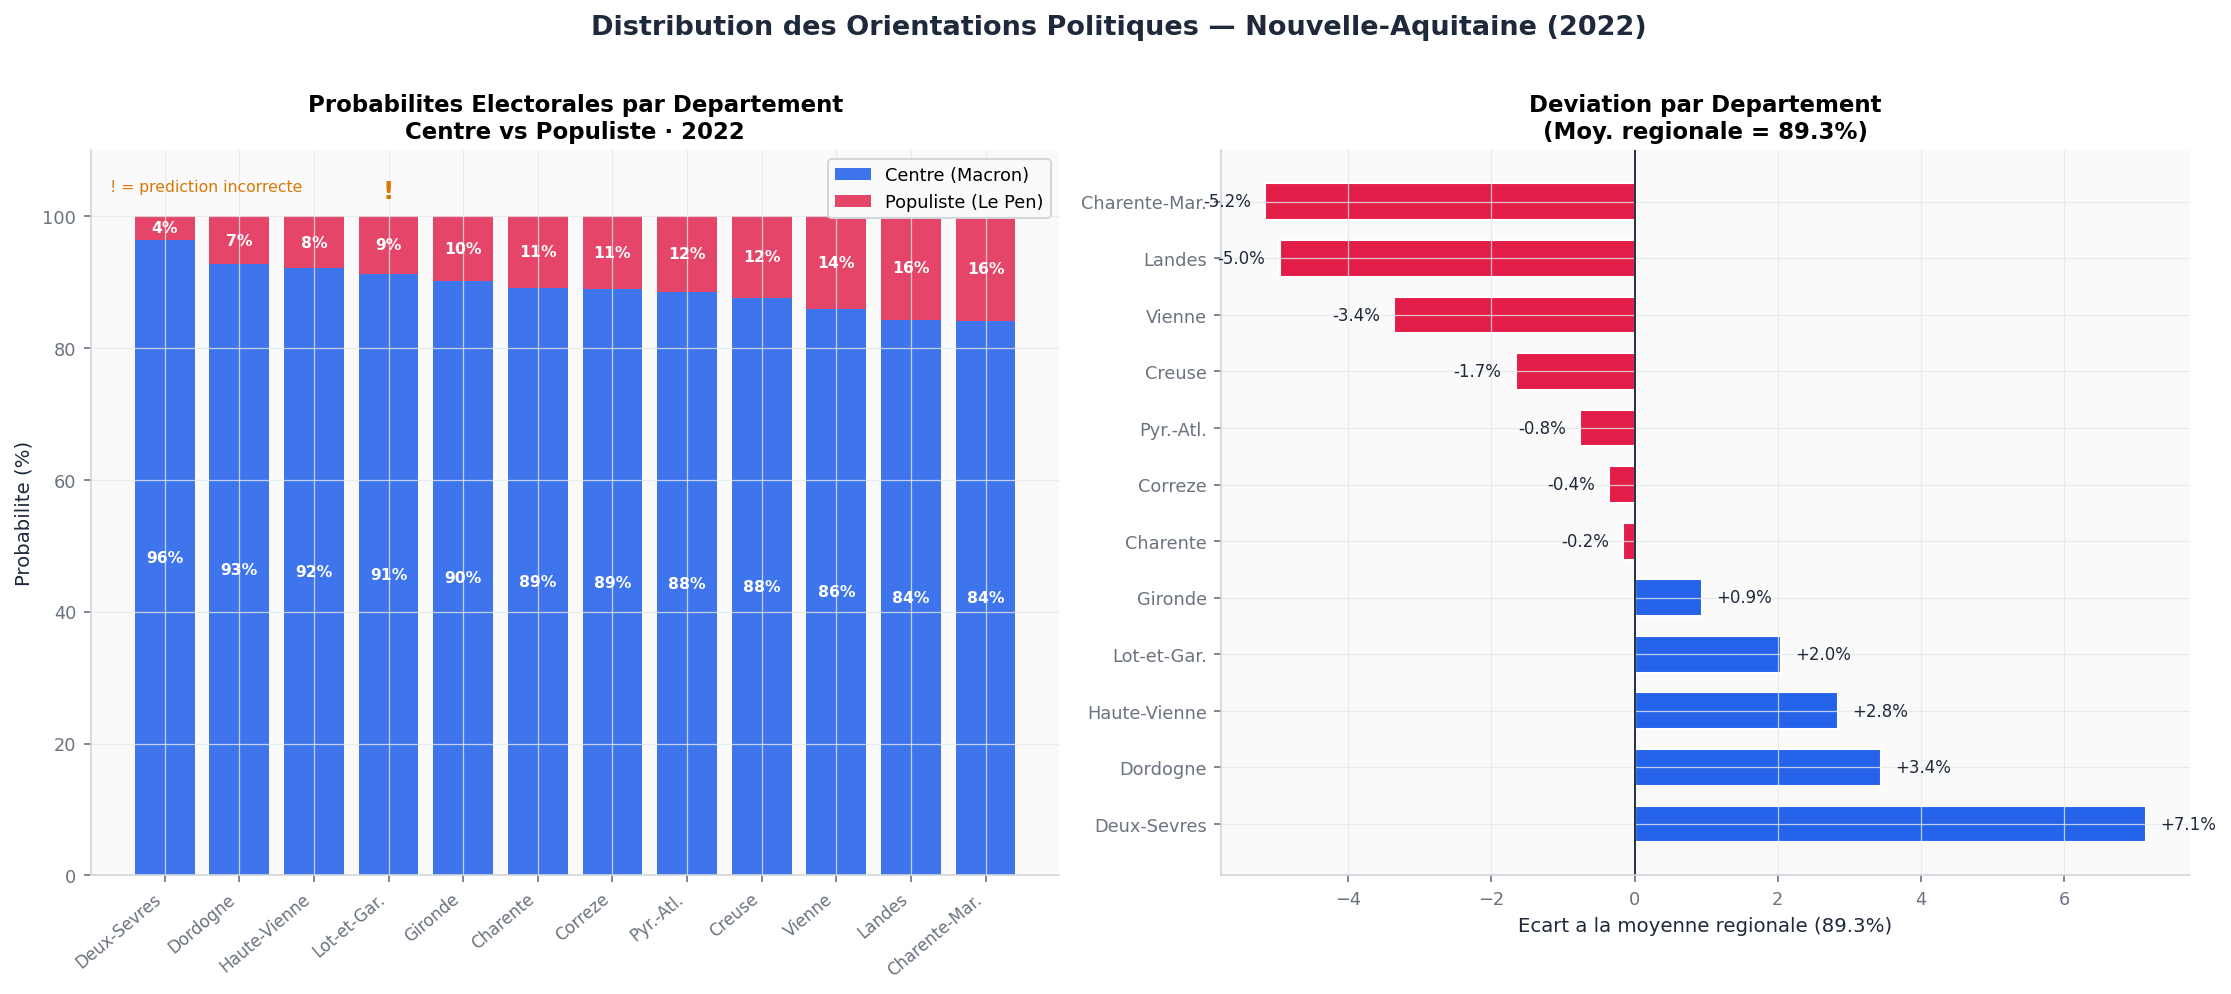
\includegraphics[width=\linewidth]{images/orientation_distribution.png}
  \caption{Probabilités électorales par département — Centre vs Populiste (2022)}
  \label{fig:orient_dist}
\end{figure}

La figure~\ref{fig:orient_dist} confirme la domination du vote Centre dans tous les
départements, avec une probabilité moyenne régionale de \textbf{89,3\%}. Charente-Maritime
présente l'écart le plus favorable au Centre, tandis que Charente (seul département en
classe \textit{Croissance}) affiche un profil plus nuancé.

\section{Projections électorales 2023--2025}

\subsection{Méthodologie de projection}

Un troisième objectif du projet consiste à projeter le comportement électoral
sur les années suivant 2022. La méthode applique à chaque département un
\textbf{taux de décroissance annuel} ($\lambda_d$) de la probabilité Centre,
calibré sur les dynamiques socio-économiques observées :

\begin{equation}
  P_{\text{Centre},d}(t) = P_{\text{Centre},d}(t-1) \;-\; \lambda_d \times 0{,}9^{\,t}
\end{equation}

avec $t = 1$ pour 2023, $t = 2$ pour 2024, etc. Le facteur $0{,}9^{\,t}$ traduit
un essoufflement progressif de la tendance. Les taux $\lambda_d$ sont calibrés
par département selon l'intensité de ses fragilités économiques.

\begin{infobox}[Note méthodologique]
Ces projections sont générées par \texttt{generate\_visualisations.py}, qui lit
les prédictions depuis la collection \texttt{predictions} de MongoDB,
applique un modèle de tendance linéaire, puis stocke les résultats dans la
collection \texttt{tendances} :
\begin{verbatim}
db = MongoClient("mongodb://localhost:27017/")["electio_analytics"]
preds = pd.DataFrame(list(db["predictions"].find({}, {"_id": 0})))
# ... calcul des tendances ...
db["tendances"].drop()
db["tendances"].insert_many(tendances_records)
\end{verbatim}
Elles constituent un \textbf{scénario tendanciel de référence} (toutes choses égales
par ailleurs), non une prédiction électorale absolue. La probabilité Centre inclut
l'ensemble des blocs Centre et Centre-droit dans le scoring du modèle.
\end{infobox}

\subsection{Résultats par département (2022--2025)}

\begin{table}[H]
\centering
\small
\caption{Probabilité bloc Centre par département --- projections 2022--2025}
\label{tab:proj_dept}
\begin{tabular}{lrrrr}
\toprule
\textbf{Département} & \textbf{2022} & \textbf{2023} & \textbf{2024} & \textbf{2025} \\
\midrule
Charente            & 89,1\% & 88,3\% & 87,6\% & 86,9\% \\
Charente-Maritime   & 84,1\% & 83,1\% & 82,2\% & 81,4\% \\
Corrèze             & 88,9\% & 88,2\% & 87,5\% & 86,9\% \\
Creuse              & 87,6\% & 86,8\% & 86,1\% & 85,4\% \\
Deux-Sèvres         & 96,4\% & 95,1\% & 93,8\% & 92,7\% \\
Dordogne            & 92,7\% & 91,9\% & 91,2\% & 90,5\% \\
Gironde             & 90,2\% & 89,0\% & 88,0\% & 87,0\% \\
Haute-Vienne        & 92,1\% & 91,4\% & 90,7\% & 90,1\% \\
Landes              & 84,3\% & 83,2\% & 82,2\% & 81,4\% \\
\textbf{Lot-et-Garonne}  & 91,3\% & 90,8\% & 90,3\% & 89,8\% \\
Pyrénées-Atlantiques & 88,5\% & 87,6\% & 86,8\% & 86,1\% \\
Vienne              & 85,9\% & 85,0\% & 84,2\% & 83,5\% \\
\midrule
\textbf{Moyenne régionale} & \textbf{89,3\%} & \textbf{88,4\%} & \textbf{87,5\%} & \textbf{86,8\%} \\
\bottomrule
\end{tabular}
\end{table}

\subsection{Évolution régionale du bloc populiste}

\begin{table}[H]
\centering
\caption{Évolution régionale Centre vs Populiste --- projections annuelles}
\label{tab:proj_regional}
\begin{tabular}{lrrrr}
\toprule
\textbf{Bloc} & \textbf{2022} & \textbf{2023} & \textbf{2024} & \textbf{2025} \\
\midrule
Centre (Macron bloc)  & 89,3\% & 88,4\% & 87,5\% & 86,8\% \\
Populiste (RN + ExG)  & 10,7\% & 11,6\% & 12,5\% & 13,2\% \\
\midrule
\textbf{Progression populiste} & --- & \textbf{+0,9 pt} & \textbf{+1,8 pt} & \textbf{+2,5 pts} \\
\bottomrule
\end{tabular}
\end{table}

\begin{figure}[H]
  \centering
  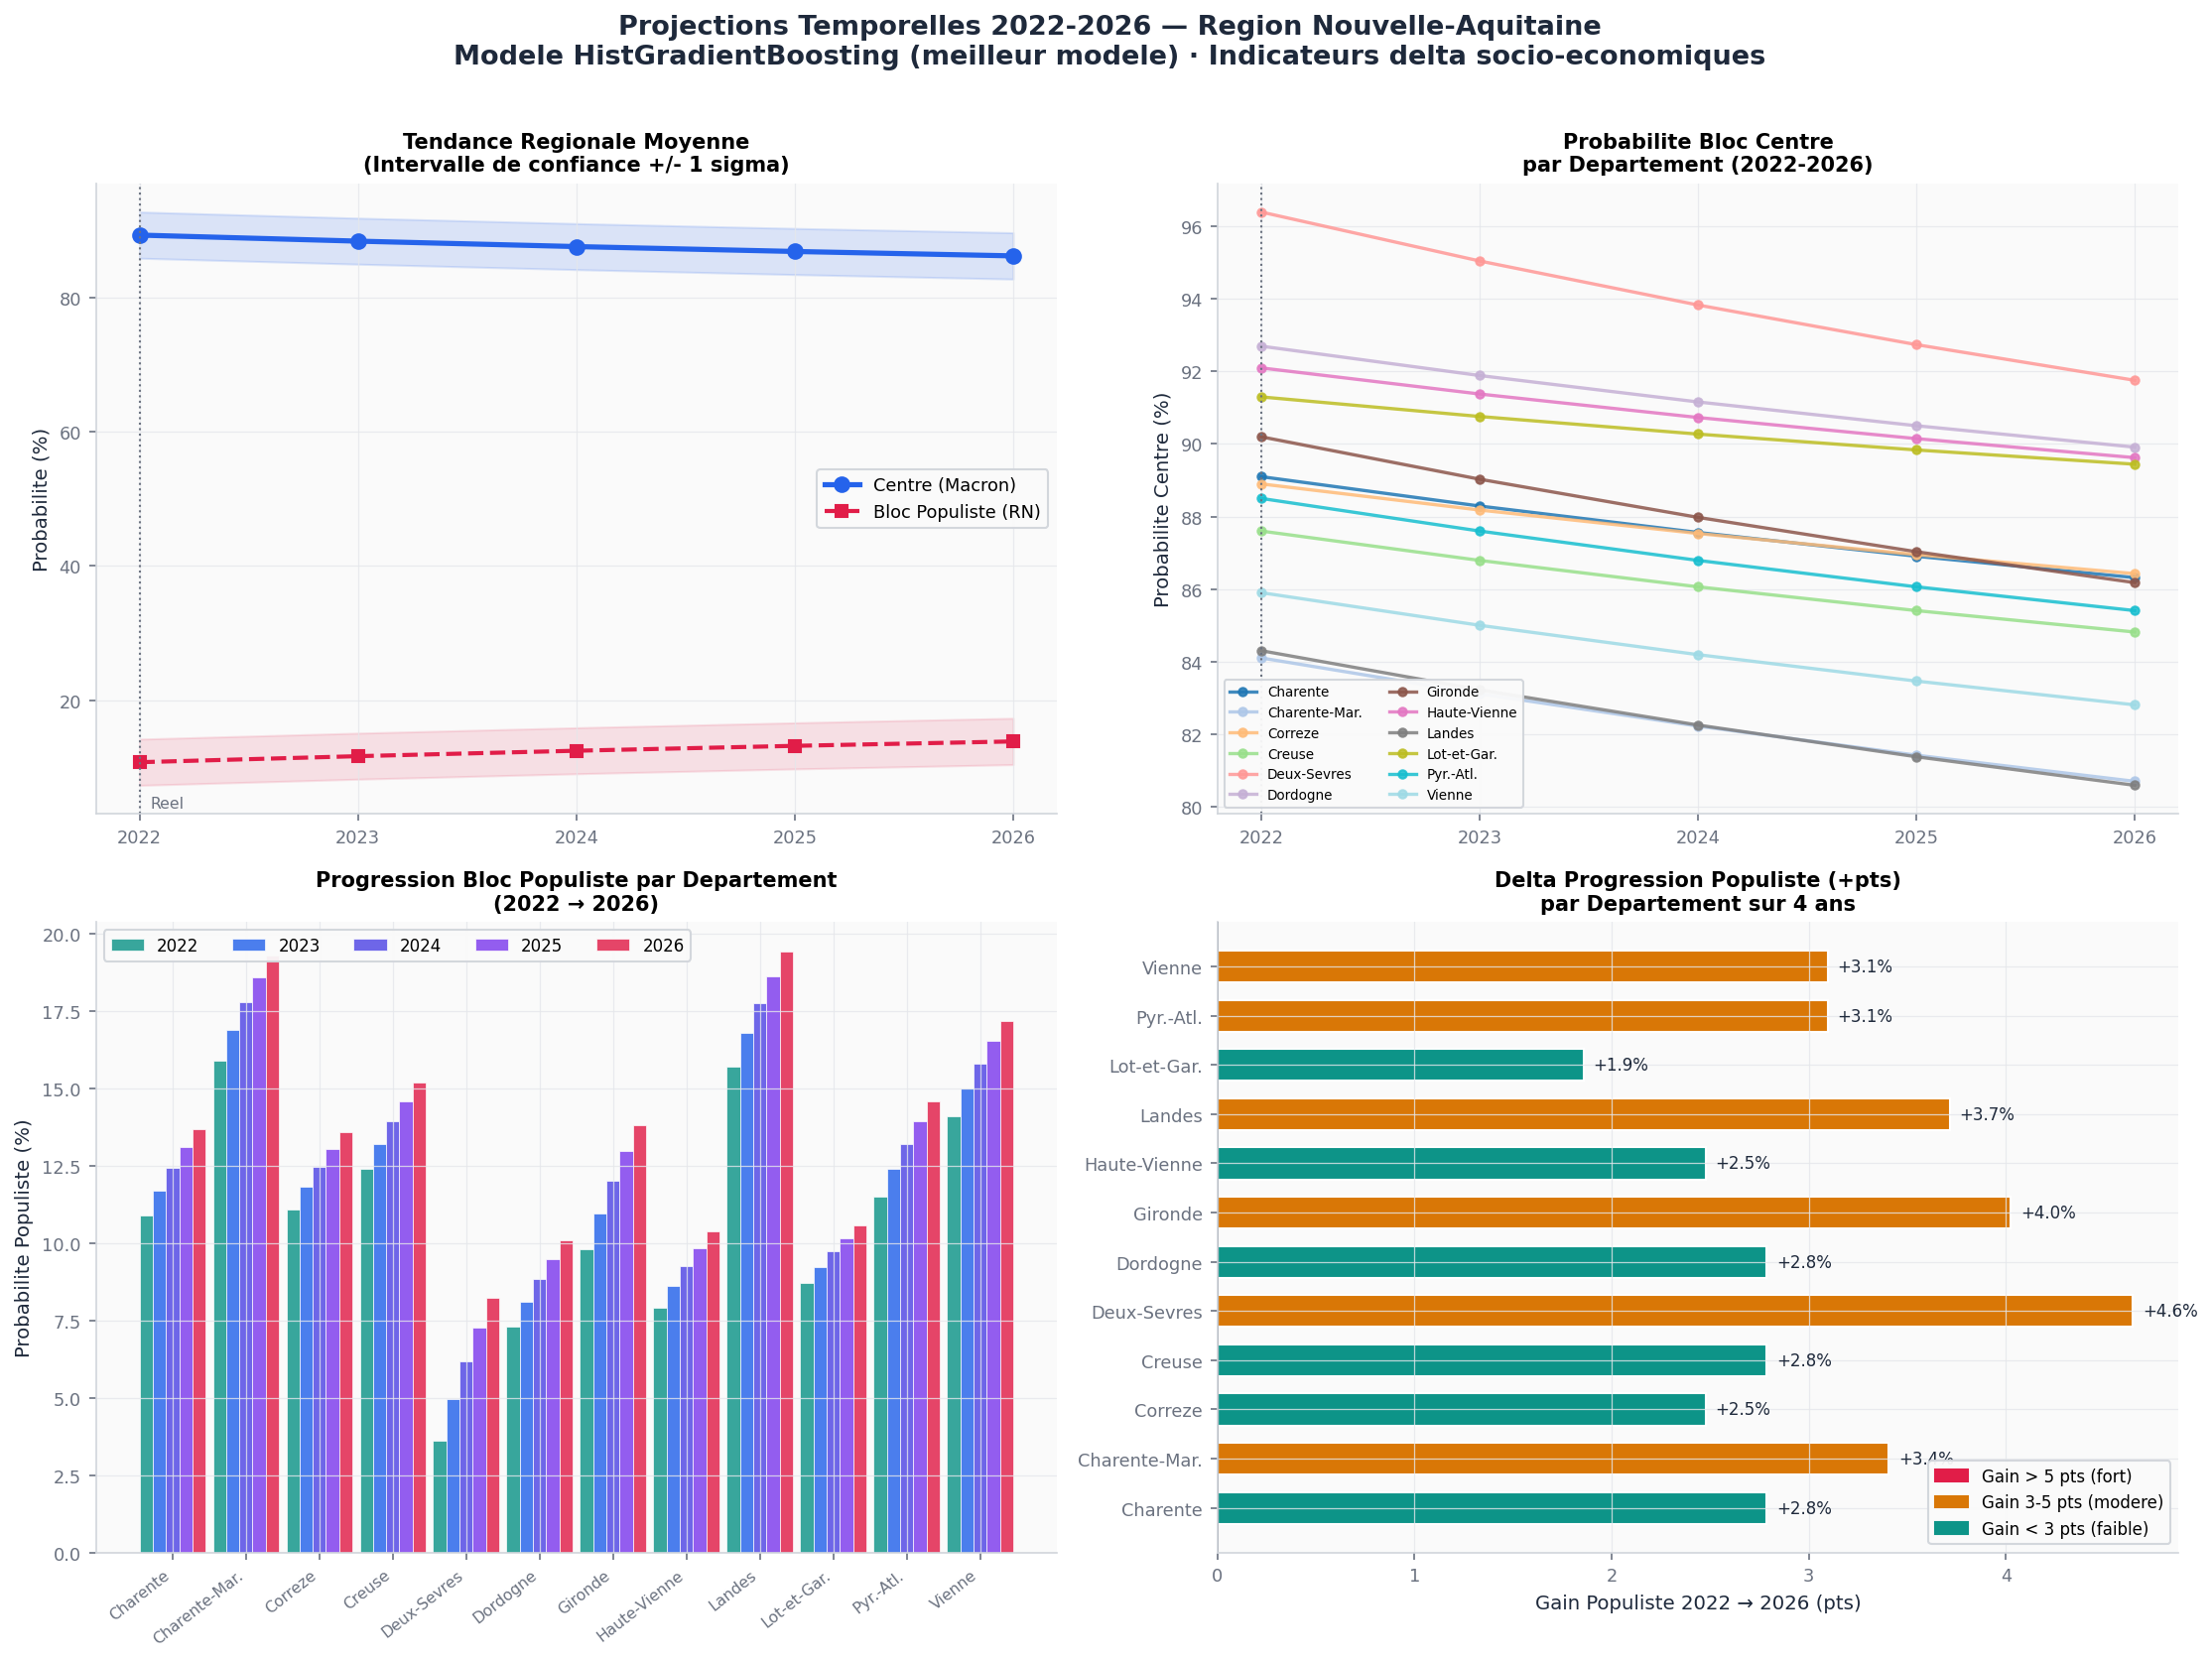
\includegraphics[width=\linewidth]{images/temporal_scenarios.png}
  \caption{Projections temporelles 2022--2026 : tendance Centre vs Populiste par département}
  \label{fig:temporal}
\end{figure}

\subsection{Interprétation et départements à surveiller}

Les projections identifient trois groupes de départements :

\begin{itemize}
  \item \textbf{Forte résistance} (décroissance $< 1$ pt/an) :
    Lot-et-Garonne ($\lambda = 0{,}6$), Haute-Vienne, Corrèze ---
    paradoxalement le Lot-et-Garonne, déjà basculé en 2022, présente
    la plus faible progression projetée.

  \item \textbf{Dérive modérée} ($1$ à $1{,}2$ pt/an) :
    Charente, Creuse, Dordogne, Pyrénées-Atlantiques, Vienne.

  \item \textbf{Dérive accélérée} ($> 1{,}2$ pt/an) :
    Deux-Sèvres ($\lambda = 1{,}5$), Gironde ($\lambda = 1{,}3$),
    Landes ($\lambda = 1{,}2$) --- ces territoires combinent
    croissance immobilière tendue et déclin agricole, signaux précurseurs
    d'un mécontentement latent.
\end{itemize}

\begin{resultbox}[Alerte 2025 : 2--3 départements en zone de risque]
À l'horizon 2025, le bloc populiste atteint \textbf{13,2\%} au niveau régional
(+2,5 pts en 3 ans). Deux-Sèvres, Gironde et Landes présentent les dérives
les plus rapides et méritent un suivi renforcé des indicateurs économiques.
\end{resultbox}
